\chapter{Introduction}
% Das autonome Fahren und die Vernetzung von Fahrzeugen mit Ihrer Umwelt sind zusammen mit der Elektromobilität die meistdiskutierten Themen der Automobilbranche.
% Zu Recht: Autonomes Fahren besitzt das Potenzial, im Mobilitätsmarkt völlig neue Strukturen entstehen zu lassen.
``Autonomous driving and the networking of vehicles with their environment are, together with electromobility, the most frequently discussed topics in the automotive sector.
Rightly so: Autonomous driving has the potential to create completely new structures in the mobility market.''
\footnote{\url{https://www2.deloitte.com/de/de/pages/consumer-industrial-products/articles/autonomes-fahren-in-deutschland.html} (03/09/2017)}

% So ebenfalls die Technische Hochschule Chalmers welche ergänzend zu Volvos “DriveMe” Projekt das Projekt
% “CampusShuttle” initiiert hat, “CampusShuttle” ist ein interdisziplinäres Forschungsprojekt der Technischen Hochschule Chalmers und der Universität Göteborg.
% Das Projekt ist dabei im ReVeRe (Chalmers Research Vehicle Resource) angesiedelt. Die Vision ist dabei ein selbstfahrendes Auto zwischen den beiden Campus der Technische Hochschule Chalmers.
So also, the Chalmers University of Technology, which has also initiated the project "CampusShuttle" in addition to Volvos' "DriveMe" project, 
is an interdisciplinary and cooperative research project at the Chalmers University of Technology and the University of Gothenburg.
The project is located in the ReVeRe (Chalmers Research Vehicle Resource). The vision is a self-driving car between the two campuses of Chalmers.

% Dabei soll, im Rahmen des Projekts, das Fahrzeug in verschiedenen Verkehrsszenarien untersucht werden. Der Fokus liegt dabei besonders auf den Stadtverkehr, das Fahrzeug muss dabei nicht
% nur in der Lage sein mit anderen Autos zu interagieren, sondern ebenfalls mit Straßenbahnen, Bussen, Fahrrädern aund allen Anderen Verkehrsteilnehmern sicher agieren. 
Within the scope of the project, the vehicle is to be examined in various traffic scenarios. The focus is on urban transport and the vehicle must not only be able to interact with other cars, 
but also be safe with trams, buses, bicycles and all other traffic users.

\section{Initial Situation}


\subsection{Test Platform}

\begin{figure}[!ht]
%\begin{center}
\caption{Test Platform Snowfox}
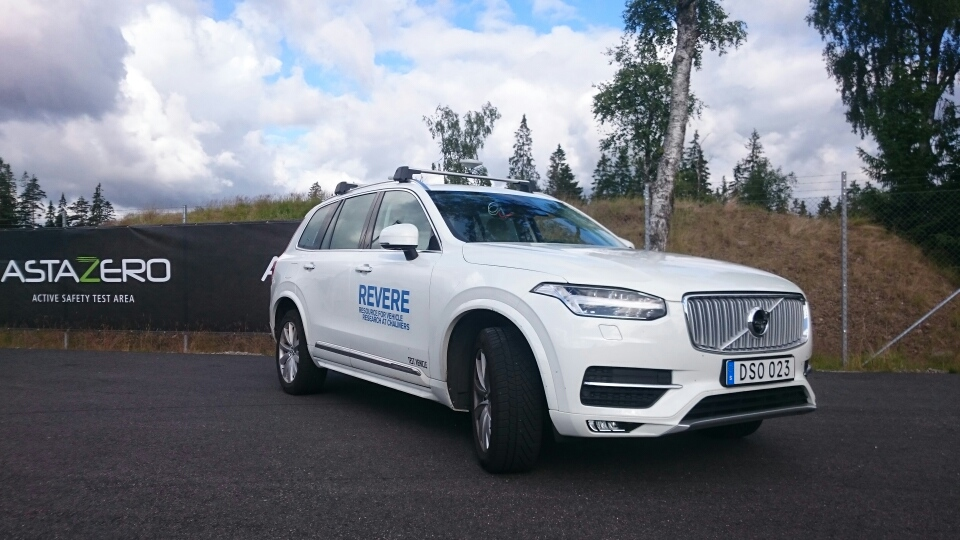
\includegraphics[width=\columnwidth]{bilder/snowfox.jpg}
\label{snowfox}
%\end{center}
\end{figure}

% Die in dieser Arbeit genutze Testplatform ist ein Volvo XC90 (2015) SUV, gennate Snowfox (siehe \cref{snowfox}). Diese Testpaltform ist mit vielen Sensoren zur Umfeldwarnehmung ausgestattet.
% Dazu zählen fünf Radar Sensoren, rund um das Fahrzeug. Wobei das Front Radar über eine Größere Reichweite verfügt. Sowie eine
% Stereo Kamera und ein Velodyne VLP-16 LiDAR. Die Anordnung der Sensoren kann \cref{platform} entnommen werden.

The test platform used in this work is a Volvo XC90 (2015) SUV, named Snowfox (see \cref{snowfox}). 
This test platform is equipped with many sensors for environmental monitoring. This includes five radar sensors, all around the vehicle, where front radar has a wider range.
As well as a stereo camera and a Velodyne VLP-16 LiDAR. The arrangement of the sensors can be taken from \cref{platform}.


\begin{figure}[!ht]
%\begin{center}
\caption{Snowfox Sensors}
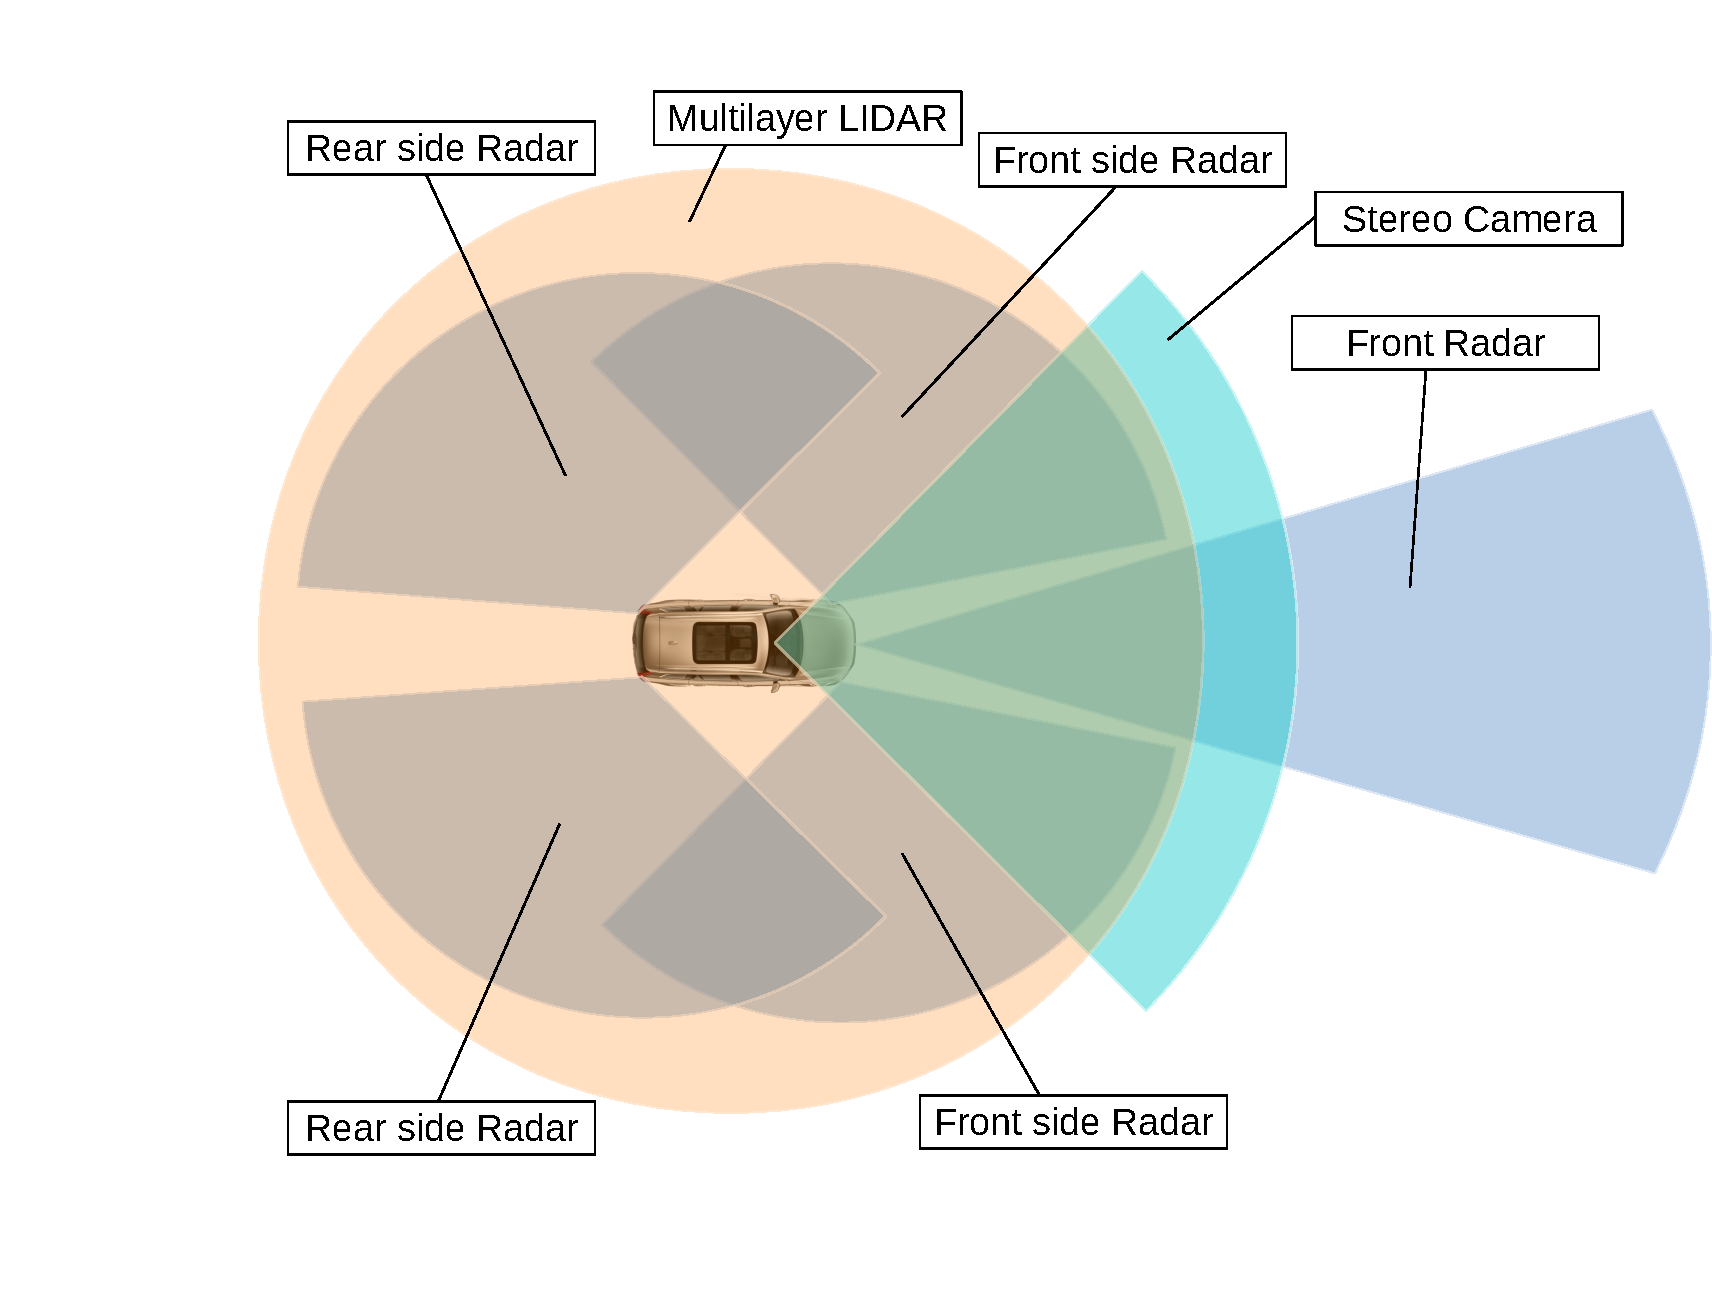
\includegraphics[width=\columnwidth]{sensors.pdf}
\label{platform}
%\end{center}
\end{figure}

% Zusätlich zur Umfeldsensorik und der serienmäßgigen Fahrzeugsensorik (z.B. Odometer, Interialsensorik) ist im Fahrzeug ein Applanix POS LV verbaut.
% Zu Zeitpunkt des Verfassens dieser Arbeit war es leider noch nicht möglich auf die Radarsensoren und die Stereokamera zuzugreifen. 
% Daher werden im folgenden lediglich der Velodyne LiDAR und das Applanix System genauer beschrieben.
A Applanix POS LV is installed in the vehicle in addition to the environmental sensor system and the standard vehicle sensors (for example odometer, intertial sensors).
At the time of writing this work, it was unfortunately not yet possible to access the radar sensors and the stereo camera.
Therefore, only the Velodyne LiDAR and the Applanix system will be described in detail.

\subsubsection{Velodyne VLP-16 LiDAR}
% Der Velodyne VLP-16 ist ein 360 Grad 3D Laserscannermit einer Rotationsgeschwindigkeit von 5 bis 20 Umdrehungen pro Sekunde \cite{manVEL}. Er bietet ein vertikales FOV von 30 Grad, bei 2 Grad Auflösung.
% Mit einer Reichweite von 100m kann er einen Umkreis von 200m Durchmesser abdecken. Weiterhin kann der VLP-16 mit dem Applanix POS LV syncronisiert werden, was eine jitterarme Zeimessung ermöglicht.
% Eine weiter Funktion des Velodyne Sensors, ist das er auf verschiedene Messimpulse reagieren kann. Durch die Auswertung des letzten Impulses statt des Stärksten Impulses ist es Möglich durch Transparent Objekte zu sehen.
% Das ermöglicht uns im späteren Verlauf die Breite des Fahrzeues zu ermitteln, da der Velodyne durch die Glasfenster des Fahrzeues blicken kann.
% Bei einer eingestellten Geschwindigkeit von 10Hz liefert der VLP-16 eine Auflösung von 0.2 Grad bei einer Abreichung von +-3cm. Der VLP-16 ist mittig auf dem Dach des XC90 moniert, um eine möglichst hohe Positionierung
% zu erreichen, die eine Rundumsicht umd Das Fahrzeug zu erreichen. Zu beachten ist, das diese Ausrichtung für den Sensor denkbar ungünstig ist, da der Sensor ein vertikales
% Sichtfeld von -15 bis +15 Grad hat. Dadurch sind nachezu alle messungen über Null grad quasi nutzlos. Der blick auf die Herstellerseite
% \footnote{\url{http://velodyneLiDAR.com/vlp-16.html} (03/09/2017)}
% verrät, das Der VLP-16 aunteranderem auf die verwendung mit Drohnen hin konstuiert wurde, während der Größere HDL64E
% \footnote{\url{http://velodyneLiDAR.com/hdl-64e.html} (03/09/2017)}
% explizit für den Urbanen Automotivebereich beworben wird, und über ein Sichtfeld von +2 bis -24.9 Grad verfügt und somit für die Verwendung im
% Automotive bereich geeigneter erscheint. Die dabei entstehenden Probleme werden später diskutiert.

The Velodyne VLP-16 is a 360 degree 3D laser scanner with a rotational speed of 5 to 20 revolutions per second \cite{manVEL}.
It provides a vertical FOV of 30 degrees, at 2 degrees resolution.
With a range of 100m it can cover a circumference of 200m diameter. 
Furthermore, the VLP-16 can be syncronized with the Applanix POS LV, which allows a low-jitter signal. 
A further function of the Velodyne sensor is that it can react to different measuring pulses. 
By evaluating the last pulse instead of the strongest pulse it is possible to see through transparent objects. 
This allows us to determine the width of the vehicle in a later part of this work, as the Velodyne can look through the glass windows of the vehicle. 
At a set speed of 10Hz, the VLP-16 provides a resolution of 0.2 degrees with a variance of +- 3cm. 
The VLP-16 is centered on the roof of the XC90 in order to achieve the highest possible positioning to achieve a panoramic view of the vehicle.
It is important to note that this alignment is unacceptable to the sensor because the sensor has a vertical field of view of -15 to +15 degrees.
As a result, all measurements over zero degrees are practically useless. The view of the manufacturer side
\footnote{\url{http://velodyneLiDAR.com/vlp-16.html} (03/09/2017)}
reveals that the VLP-16 has been constituted for use with drones, while the larger HDL64E
\footnote{\url{http://velodyneLiDAR.com/hdl-64e.html} (03/09/2017)}
is advertised explicitly for the urban automotive sector, and has a field of view of +2 to -24.9 degrees and thus for use in the
Automotive sector appears to be more appropriate. The resulting problems will be discussed later.






\subsubsection{Applanix POS LV}
% Das POS LV ist ein kompaktes Positions- und Orientierungssystem. Es Offeriert stabile, zuverlässige und reproduzierbare Positionierungslösungen für landgestützte Fahrzeuganwendungen.
% Das POS LV liefert dabei eine Inertialsensork und Odometrie gestützte Positionsmessung mit einer Genauigkeit von bis zu 0.3m (bis zu 0.035m bei verwendung von der der RTK - Korrektur).
% Im weiteren Verlauf wird außerdem das vom POS LV gelieferte Heading genutzt, welches eine Genauigkeit von 0.2 Grad liefert. Auch nach ausfall des GPS-Signals kann das POS-LV durch sein
% Odeomerter und der Inertialsensork eine Position liefern. Diese wird jedoch über die Zeit schlechter, so das 60Sek nach Ausfall des GPS-Signals nich eine Genauigkeit von 2.51m erwartet
% werden kann.\cite{manAP}
The POS LV is a compact position and orientation system. It offers stable, reliable and reproducible positioning solutions for land-based vehicle applications. The POS LV provides an 
inertial sensor and odometry based position measurement with an accuracy of up to 0.3m (up to 0.035m when using the RTK correction).
Furthermore, the heading delivered by the POS LV is also used, which provides an accuracy of 0.2 degrees. Even after losing the GPS signal,
the POS-LV can provide a position through its odometer and the inertial sensor. However, this will deteriorate over time so that an accuracy of 2.51m
can be expected 60 seconds after the GPS signal is lost. \cite{manAP}


\section{Research Goal}
% Da das Autonome Fahren ein sehr weites, indisziplinäres thema ist, ist es Offensichtlich. das nicht alles in dieser Arbreit abgehandelt werden kann.
% Im Rahmen der darpah Chalenge wurden beiteits viele Veröffentlichungen zu diesem Thema erstellet.
% Was im rahmen dieser Veröffenticghungten noch nicht berhandelt wurde, sit dei Handhabung von Kreisverkehre, mit atonomen Fahrzeugen.
% Ziel dieser Arbeit ist es Daher zu analysieren, welche Sensorausstattung für die beobachtung von Kreisverkehren vonnöten ist, bzw. ob die vorhandenne Sensorausstattung des ReVeRe Testfahrzeuges Snowfox
% als ausreichend betrachtet werden kann.
Since autonomous driving is a very wide, indisciplinary subject, it is obvious, that not everything can be dealt within this work.
Within the scope of \acs{DARPA} Chalenge many papers were published on this subject. What has not yet been explicitly discussed in these publications
is the explicit handling of roundabouts, with autonomic vehicles, also the author is not aware of any further publications. 
So the aim of this thesis is therefore to analyze what sensor equipment is necessary for the observation of roundabouts,
or whether the existing sensor equipment of the ReVeRe test vehicle Snowfox can be regarded as sufficient.

